We compare our custom tensor contraction algorithm to the einsum engines of PyTorch and Numpy as well as to the np\_mm backend. To evaluate the performance of each engine, we use two different sets of problems: First, we test all four engines on simple pairwise tensor contractions with different structural characteristics. Second, we evaluate the four einsum engines on real-world einsum expressions.\\
\textcite{blacher2024einsum} point out that most current tensor libraries are optimized for a limited range of tensor operations, particularly those involving large, dense tensors. However, real-world applications often require a much broader variety of tensor operations, which can cause performance issues. To solve this problem, they present the einsum\_benchmark dataset that includes a wide range of tensor operations and covers the diverse types of operations used in practice. To address this issue, we assess the performance of all four implementations on 28 real-world problems from that dataset.\\
We measure the iterations per second for all experiments, that is, how often a given einsum expression can be executed within one second. \\
The experiments are performed on a machine with
an Intel i5-7200U 2-core processor running Ubuntu 22.04-1 with 8 GB of RAM.
Each core has a base frequency of 2.5 GHz and a max boost frequency of 3.1 GHz. The evaluation is done in
Python 3.12.8 with PyTorch 2.5.1 and Numpy 2.2.1.

\section{Experiments on Pairwise Tensor Contractions}
We designed four format strings for pairwise tensor contractions with or without batch dimensions, traces and arbitrary indices in different combinations as can be seen in Table \ref{tab:instance:data}.
\begin{table}[H]
    \caption{Format string and properties of the four einsum expressions.}
    \label{tab:instance:data}
    \centering
    { % Apply the scriptsize font to the entire table
    \begin{tabularx}{\textwidth}{>
    {\raggedright\arraybackslash}p{3cm} >
    {\centering\arraybackslash}X >
    {\centering\arraybackslash}X >
    {\centering\arraybackslash}X}
        \toprule
        \textbf{Format String} & \textbf{Batch Dimension} & \textbf{Traces} & \textbf{Arbitrary Indices} \\
        \midrule
        aabcd,adeef$\rightarrow$dcf & yes & yes & yes  \\
        abcd,adef$\rightarrow$dbef & yes & no & yes  \\
        aabcd,adeef$\rightarrow$bcf & no  & yes & yes  \\
        abcd,adef$\rightarrow$cbef & no  & no  & no   \\
        \bottomrule
    \end{tabularx}
    }
\end{table}

\noindent To evaluate the performance of the four einsum engines across scenarios with increasing computational intensity, we repeatedly generate random tensors for each problem, increasing the dimensions for each index in each repetition. For example, the first pair of tensor generated for the einsum expression aabcd,adeef$\rightarrow$dcf has sizes (2,2,2,2,2) for both tensor $A$ and $B$, resulting in 128 floating point operations (or 2.11 floating point operations if we use a log10 scale), the second one (5,5,5,5,5), and so forth. A table with the dimension sizes and the resulting number of floating point operations for the four problems can ba found in Table~\ref{tab:dimensions} in the appendix.\\

\noindent As can be seen in Figure~\ref{flops}, our custom implementation outperformes PyTorch and Numpy for problems that contain batch dimensions, traces and arbitrary indices.
\begin{figure}[h]
    \label{flops}
    \centering
    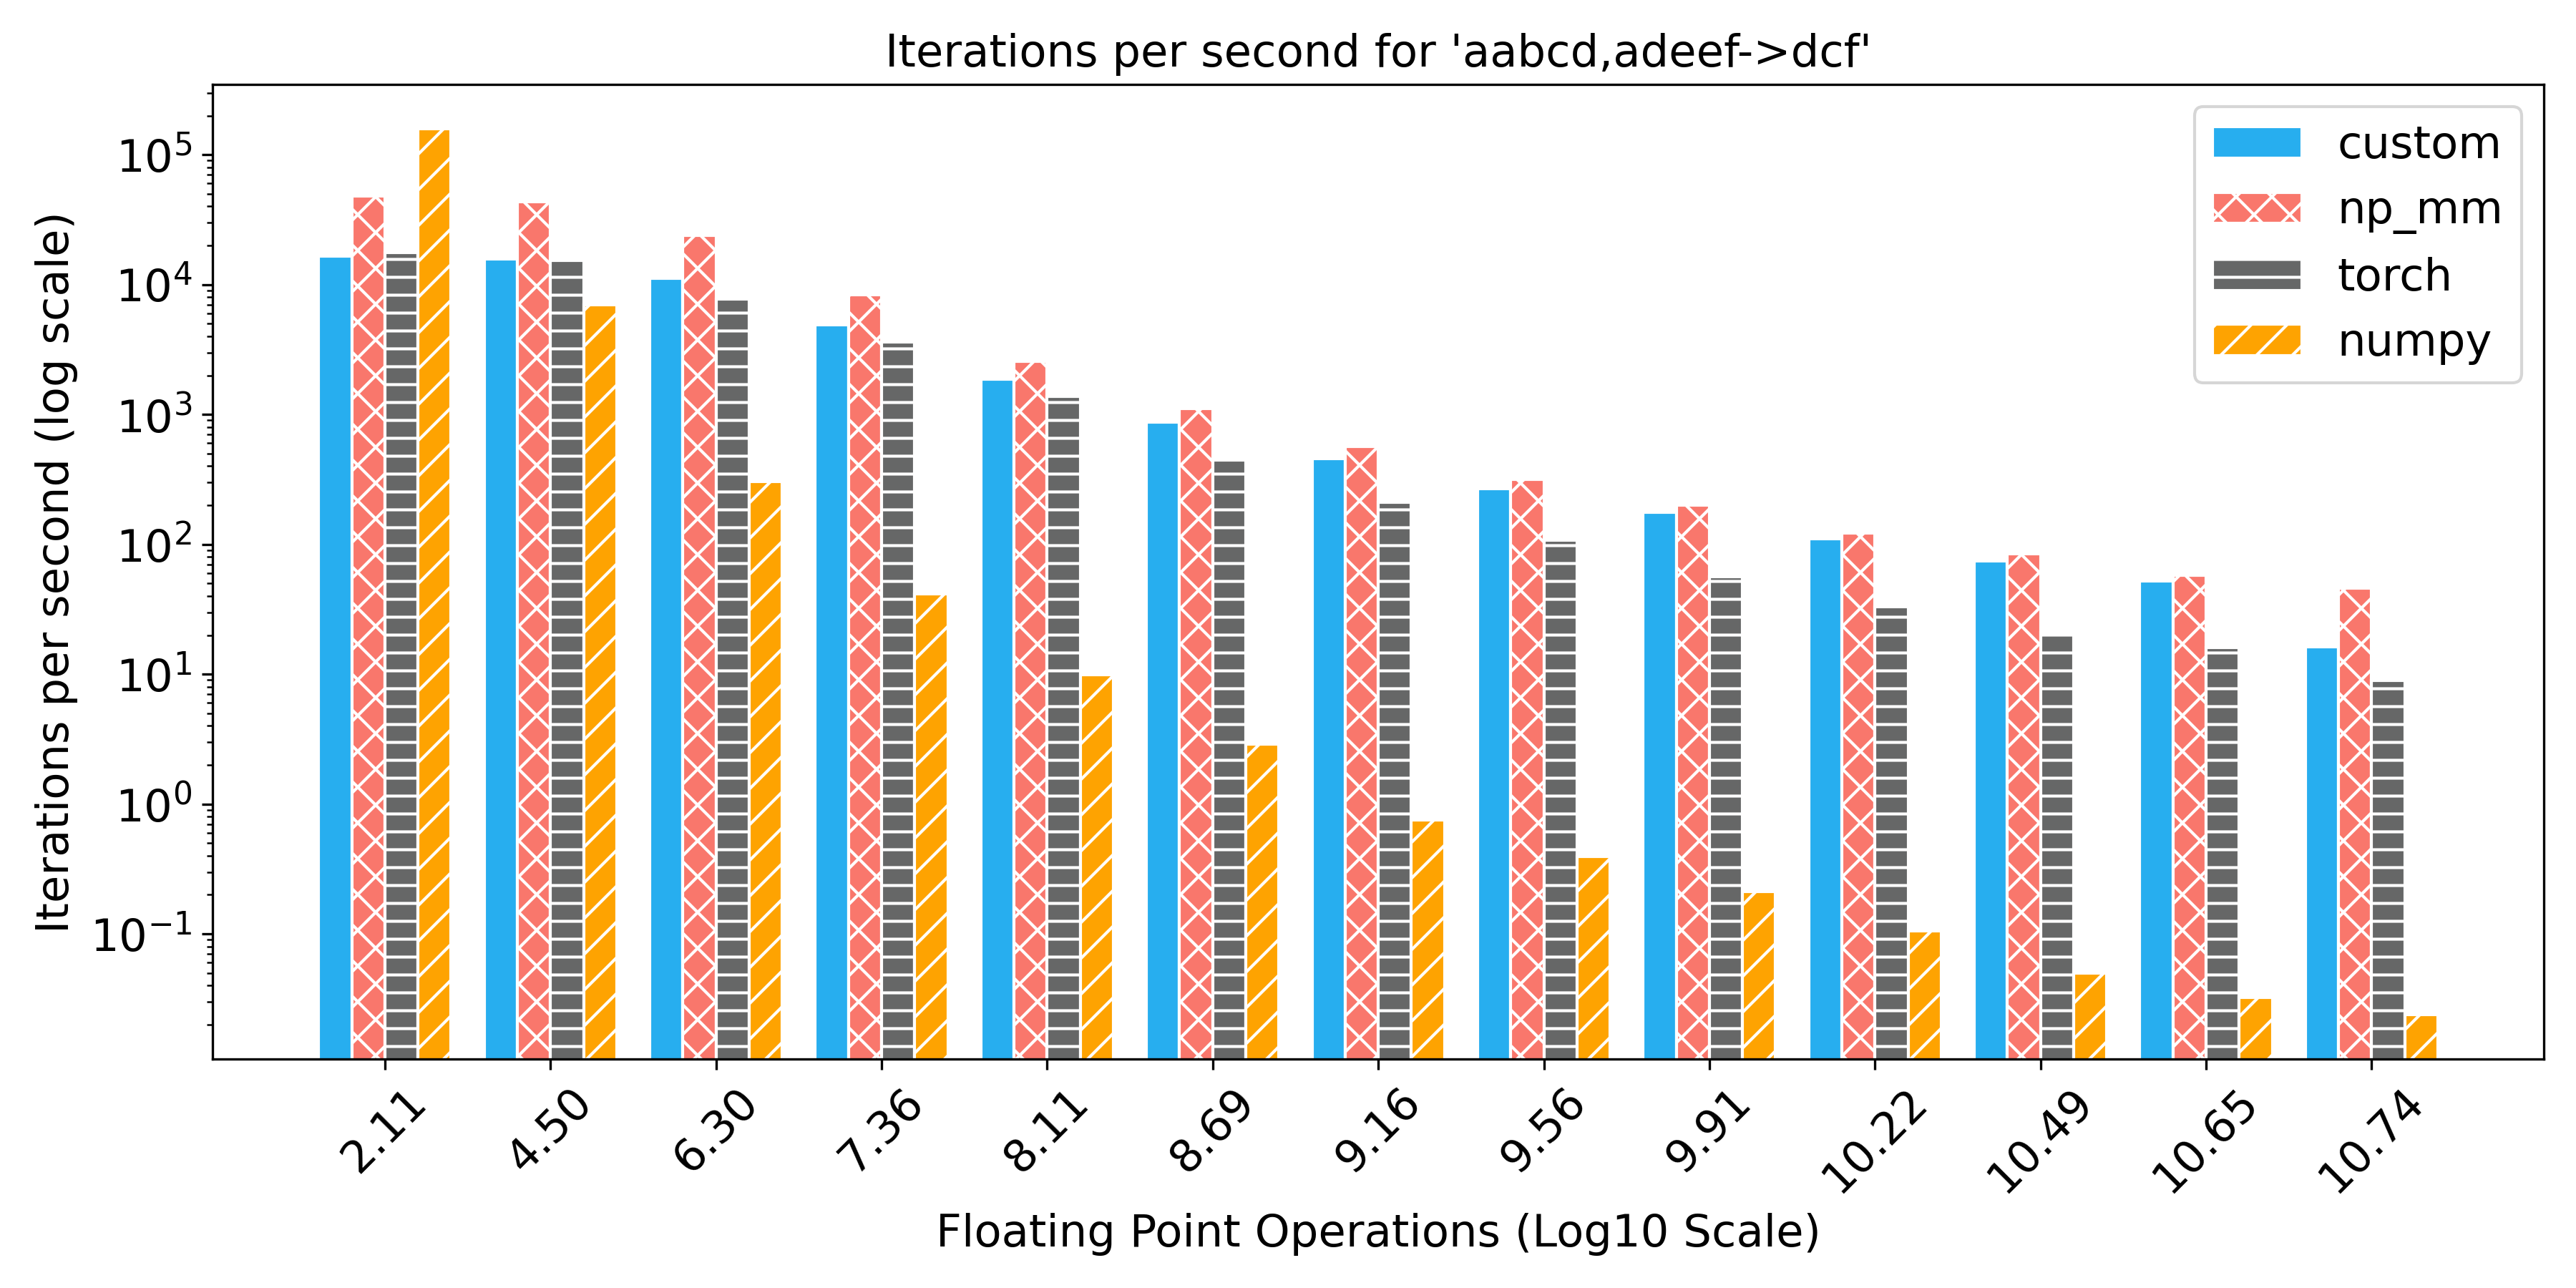
\includegraphics[width=1\textwidth]{images/aabcd_adeef__dcf.png}  % Include your image
    \caption{Performance Comparison for the pairwise contraction with batch dimensions, traces and arbitrary indices. The x-axis depicts the number of floating point operations corresponding to the gradually increased dimension sizes.}
\end{figure}

\noindent While the performance of all implementations decreases for all four problems with a growing number of floating-point operations, the rate of this degration varies. Numpy performs better than all the other backends for low counts of floating-point operations in all four contractions, as depicted in Figure~\ref{pic:all} in the appendix. However, its performance declines fastly with increasing problem size. For the largest problems, our algorithm with the np\_mm backend emerges as the most efficient method across all cases, as can be seen in Table~\ref{tab:flop_comp}.

\begin{table}[H]
    \caption{Performance comparison for the largest tensor contractions of the respective problems across the different engines, scaled to the best performance.}
    \label{tab:flop_comp}
    \centering
    {\scriptsize  % Apply the scriptsize font to the entire table
    \begin{tabularx}{\textwidth}{>
    {\raggedright\arraybackslash}p{4cm} >
    {\centering\arraybackslash}X >
    {\centering\arraybackslash}X >
    {\centering\arraybackslash}X >
    {\centering\arraybackslash}X >
    {\centering\arraybackslash}X}
        \toprule
        \textbf{\scriptsize Tensor Expression} & \textbf{\scriptsize FLOPS}& \textbf{\scriptsize Custom} & \textbf{\scriptsize np\_mm} & \textbf{\scriptsize Numpy} & \textbf{\scriptsize Torch} \\
        \midrule
        aabcd,adeef$\rightarrow$dcf &10.74& 0.35 &\textbf{ 1} & 0.00043 & 0.19 \\
        abcd,adef$\rightarrow$dbef &10.93& 0.36 &\textbf{ 1} & 0.0014  & 0.72 \\
        aabcd,adeef$\rightarrow$bcf &10.74& 0.15 &\textbf{ 1} & 0.001   & 0.42 \\
        abcd,adef$\rightarrow$cbef &10.93& 0.11 &\textbf{ 1} & 0.03    & 0.98 \\
        \bottomrule
    \end{tabularx}
    }
\end{table}


\section{Einsum Benchmark} 
We ran the 28 problems from the einsum\_benchmark dataset~\cite{blacher2024einsum} that are small enough to fit on our machine and have a non-complex data type. An overview over the properties of the einsum expressions and the performance results can be found in the appendix in Table~\ref{tab:einsum_all}.
 For our performance discussion we chose five representative problems that depict the differences between the four einsum engines. Table \ref{tab:properties} lists the relevant properties of these problems.
\begin{table}[H]
    \caption{Instance data with instance name, number of tensors and the size of the biggest intermediate tensor.}
    \label{tab:properties}
    \centering
    {\tiny  % Apply the scriptsize font to the entire table
    \begin{tabularx}{\textwidth}{>
    {\raggedright\arraybackslash}p{4cm} >
    {\centering\arraybackslash}X >
    {\centering\arraybackslash}X >
    {\centering\arraybackslash}X}
        \toprule
        \textbf{\tiny Instance Name} & \textbf{\tiny Number of Tensors} & \textbf{\tiny Biggest Intermediate Tensor} & \textbf{\tiny Data Type} \\
        \midrule
        wmc\_2023\_152 & 40489 & 16384 & float64 \\
        mc\_2023\_002  & 26556 & 131072& float64 \\
        mc\_2020\_arjun\_057 & 905 & 8388608 & int32\\
        mc\_2020\_017  & 78784 & 4194304 & int32\\
        lm\_batch\_likelihood\_sentence\_4\_12d & 84 & 39398400 & float64\\
        \bottomrule
    \end{tabularx}
    }
\end{table}

\sloppy
\noindent As can be seen in Figure \ref{e_b}, Numpy performs best for problems with small intermediate tensor sizes. Our custom algorithm is more efficient for problems with data type int\_32, while PyTorch and np\_mm are most efficient for problems with the data type double.
\begin{figure}[H]
    \centering
    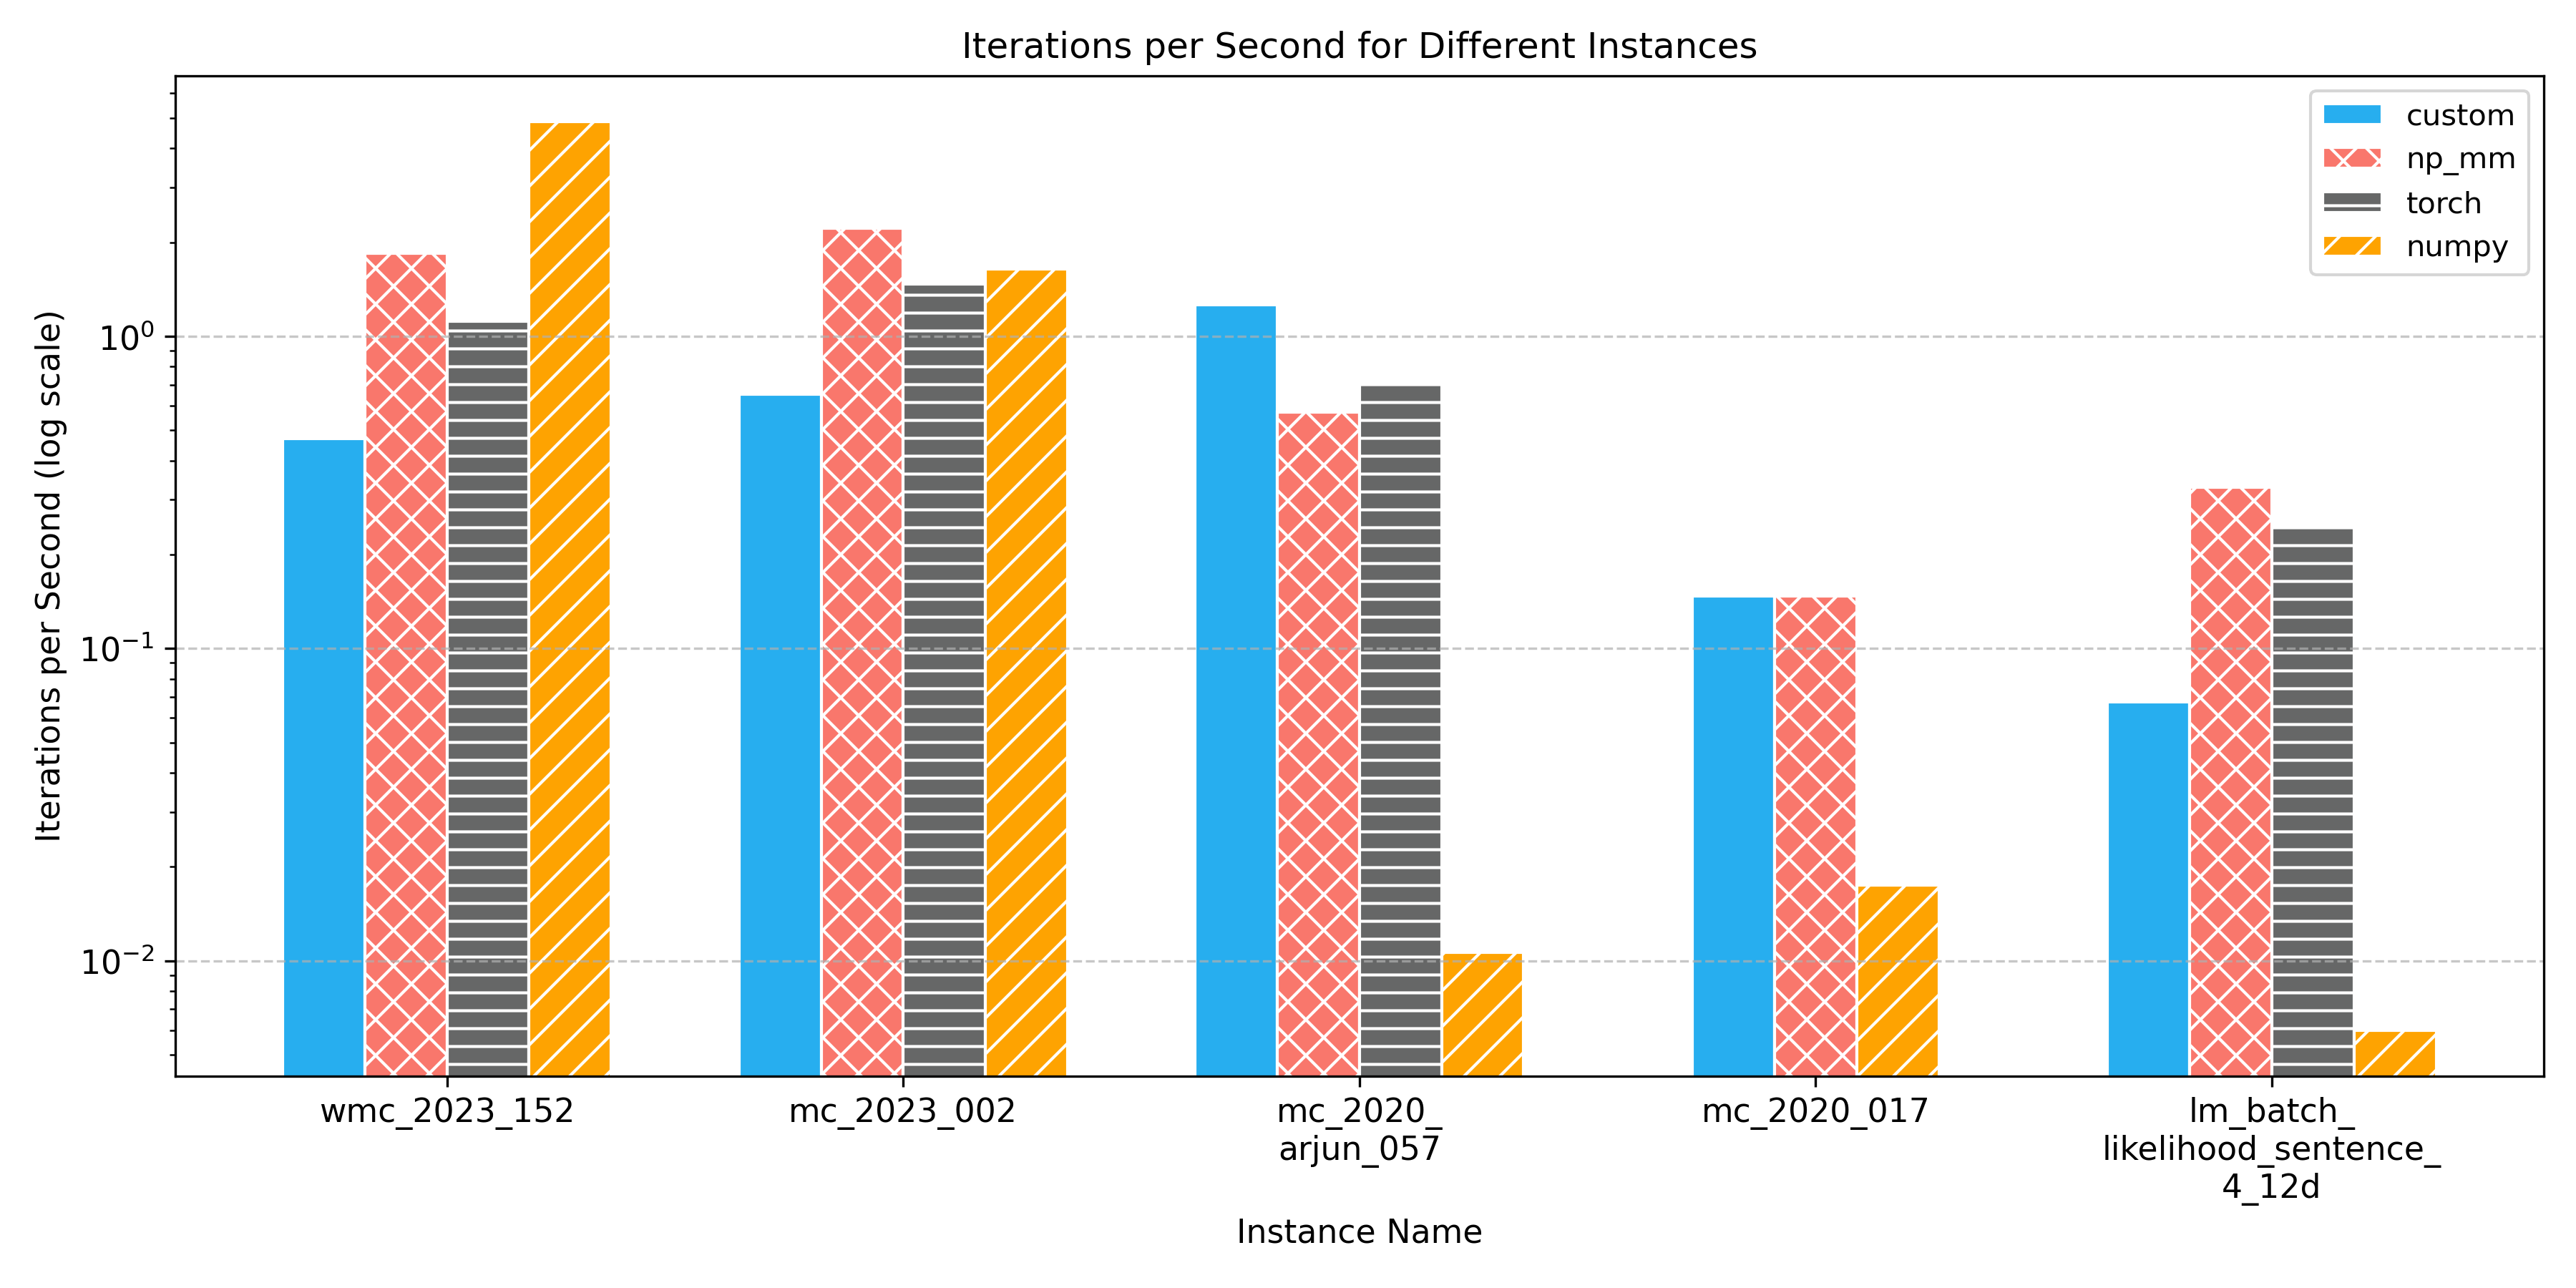
\includegraphics[width=1\textwidth]{images/einsum_five.png} 
    \caption{Performance Comparison for different problems from einsum\_benchmark~\cite{blacher2024einsum}. PyTorch was unable to compute mc\_2020\_017 due to hidden conversions from int32 to int64 during pairwise contractions.}
    \label{e_b}
\end{figure}

\noindent To further evaluate the effiency of PyTorch and np\_mm on problems with datatype double, we casted the two problems mc\_2020\_017 and mc\_2020\_arjun\_057 with datatype int\_32 to float\_64 and ran the computation again. As shown in Figure~\ref{pic:double} in the appendix, PyTorch and np\_mm both outperform the custom algorithm in this scenario.

\section{Impact of Parallelization}

\noindent To assess the impact of parallelization, we evaluated the multi-tensor contraction mc\_2020\_arjun\_046 from einsum\_benchmark~\cite{blacher2024einsum} using our custom implementation, our implementation with the np\_mm backend, and PyTorch on one and two threads. The properties of this problem can be seen in Figure~\ref{tab:arjun46_properties}. 

\begin{table}[H]
    \caption{Instance data of mc\_2020\_arjun\_046 with number of tensors and the size of the biggest intermediate tensor.}
    \label{tab:arjun46_properties}
    \centering
    {\scriptsize  % Apply the scriptsize font to the entire table
    \begin{tabularx}{\textwidth}{>
    {\raggedright\arraybackslash}p{4cm} >
    {\centering\arraybackslash}X >
    {\centering\arraybackslash}X >
    {\centering\arraybackslash}X}
        \toprule
        \textbf{\scriptsize Instance Name} & \textbf{\scriptsize Number of Tensors} & \textbf{\scriptsize Biggest Intermediate Tensor} & \textbf{\scriptsize Data Type} \\
        \midrule
        mc\_2020\_arjun\_046 & 1045 & 8388608 & int64 \\
        \bottomrule
    \end{tabularx}
    }
\end{table}
\noindent While NumPy’s batch matrix multiplication is not parallelized, our custom multi-tensor contraction shows an approximate 25\% performance improvement when increasing the thread count from one to two. PyTorch’s performance similarly improves by around 20\%. Additionally, we measured the isolated performance of our custom BMM computation. Here, the parallelization leads to an almost 50\% speed-up when scaling from one to two threads. 

\begin{figure}[H]
    \label{threads}
    \centering
    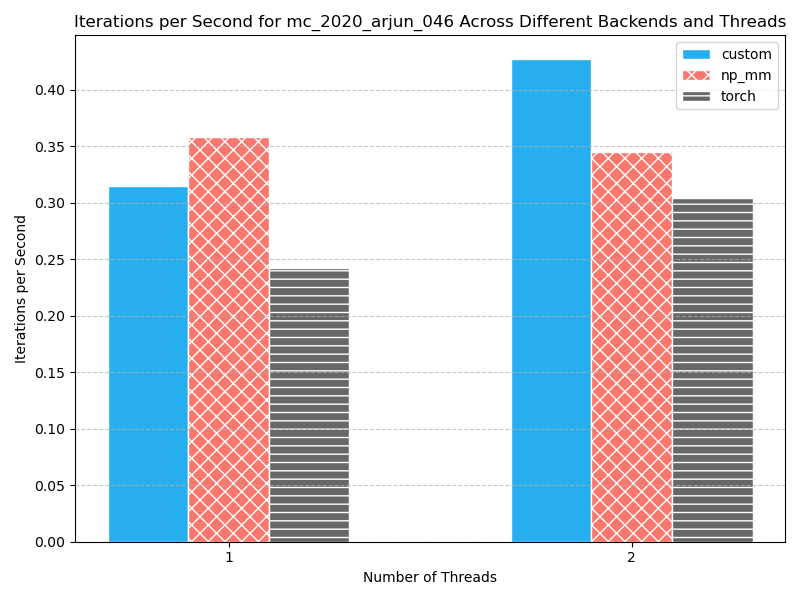
\includegraphics[width=0.6\textwidth]{images/threads.png}  % Include your image
    \caption{Iterations per second vs thread number for mc\_2020\_arjun\_046~\cite{blacher2024einsum}.}
\end{figure}